\chapter{Experiments}
\label{cha:experiments}

In this chapter, the experiments and their results are described.
The first experiment is concerned with the evaluation of the model performance on the labeled dataset that is provided by a sampling strategy.
The second one analyzes the labeled dataset that was created by the sampling strategy.
For the last experiment, an analysis and evaluation of how invalid reports can be filtered out are performed.

\section{Experiment 1: How Well do the Sampling Strategies Perform?}

This experiment aimed at evaluating how well the strategies perform, by looking into how they effect the SVM model, according to certain metrics.
The results of this experiment is used to answer the first research question.

\subsection{Method}

The active learning strategies that were evaluated are:
\begin{itemize}
    \item \textit{BSVM (BSVM)}: Described in Section~\ref{subsec:binmin}
    \item \textit{Maximum Loss Reduction with Maximum Confidence (MMC)}: Described in Section~\ref{subsec:mmc}
    \item \textit{Adaptive Active Learning (AAL)}: Described in Section~\ref{subsec:adaptive-active-learning}
\end{itemize}
The motivation behind the choice of strategies will be discussed in Chapter~\ref{cha:discussion}.

In order to provide a thorough evaluation of how well they techniques perform a set of already labeled documents was needed.
For this reason, the Reuters-21578 dataset was used, as is discussed in Section~\ref{sec:datasets}. 
The properties of the dataset, as well as a comparison between it and the clinical data provided by Sectra can be found in Section~\ref{sec:datasets}.
The dataset is common in active learning research and has been used by Brinker et al\@.~\cite{brinker2006active} and Yang et al\@.~\cite{yang2009effective}, among others.
With this dataset, the same pre-processing steps that were applied to the clinical dataset were applied to the Reuters data too.
Some modifications of this includes the stopwords, instead of a curated list of words, the unmodified list of english stopwords provided by nltk was used.
The main goal was to compare how the different techniques affected the labeled dataset, and how well an SVM model performed on it.
Optimizing the process for the particular model and dataset was therefore not the focus of the study, but instead offering a more comprehensive comparison.
With this set of labeled reports, a simulation of the labeling process was run.

The strategies need a small initial set of labeled reports which they can use to get initial predictions from the SVM model, upon which the strategies base their calculations.
The techniques were evaluated both by selecting this initial set of points at random, as well as selecting them from the clusters generated by the k-means algorithm.
Sampling from the clusters was done by iterating over the clusters and selecting an equal number of data points from each clusters.
All samples selected from a given cluster were chosen randomly amongst the members of the clusters.
Furthermore, the number of clusters selected was 25, in order to get an equal number of reports from each cluster in the different experimental settings.
Topic vectors from the topic model in Section~\ref{sec:sec:exploratory-study} was used as input to the k-means algorithm.

Since the different models may depend on the initial samples in different ways, different initial sizes were evaluated.
This is also done by Yang et al\@.~\cite{yang2009effective}.
In their paper they tried quite large initial sample sizes.
Here, the sizes evaluated are: 25, 50, 100.
The reason for this is that an large initial sample size would make it hard for the human annotator to see a difference in the class balance early on.
In each iteration, 25 labels were queried.
The ones selected every iterations were the 25 best one according to the strategy's measure.
100 iterations were run per strategy.
Making it 2500 labels that are labeled, in addition to the initial sample.
The different active learning configurations that were tried is displayed in Table~\ref{fig:active-learning-configurations}
In total there were 18 configurations, based upon the three different methods.
Every configuration was evaluated 5 times, and it is the average of those runs that are considered to be the final results.
The reasoning behind this is to reduce the effect of a single random selection.

\begin{table}
    \centering
    \begin{tabular}{|cccc|}
        \hline
        \textbf{ID} & \textbf{Active Learning Strategy} & \textbf{Initial Sampling} & \textbf{Initial Sample Size}\\
        \hline
        1 & BSVM & Random & 25\\
        2 & BSVM & Random & 50\\
        3 & BSVM & Random & 100\\
        4 & BSVM & Sampled from clusters & 25\\
        5 & BSVM & Sampled from clusters & 50\\
        6 & BSVM & Sampled from clusters & 100\\
        7 & MMC & Random & 25\\
        8 & MMC & Random & 50\\
        9 & MMC & Random & 100\\
        10 & MMC & Sampled from clusters & 25\\
        11 & MMC & Sampled from clusters & 50\\
        12 & MMC & Sampled from clusters & 100\\
        13 & AAL & Random & 25\\
        14 & AAL & Random & 50\\
        15 & AAL & Random & 100\\
        16 & AAL & Sampled from clusters & 25\\
        17 & AAL & Sampled from clusters & 50\\
        18 & AAL & Sampled from clusters & 100\\
        \hline
    \end{tabular}
    \caption{The different configurations of active learning strategies evaluated.}
    \label{fig:active-learning-configurations}
\end{table}


In each iteration, the SVM model was evaluated by being trained on the labeled data, and evaluated on the test set described in Section~\ref{sec:datasets}.
How good the SVM model's predictions are were evaluated with the following metrics:
\begin{enumerate}
    \item Accuracy
    \item Micro recall
    \item Macro recall
    \item Micro precision
    \item Macro precision
    \item Micro F1-Score
    \item Macro F1-Score
\end{enumerate}
These are described in Section~\ref{sec:evaluation-metrics} and are frequently used to compare different active learning methods, for example by Yang et al\@.~\cite{yang2009effective}, Dasgupta et al\@.~\cite{dasgupta2008hierarchical} and Li et al\@.~\cite{li2013active}.
In addition to this, how long time they take to run is compared as well.

The method here should be rather easy to replicate.
Metrics are clearly defined, and the configurations used for the different strategies are laid out.

\subsection{Results}

The first result is the SVM model's accuracy.
Its evaluation when trained on data provided by the active learning strategies with initial sample sizes of 25, 50 and 100 can be seen in Figure~\ref{fig:al-accuracy-25}, Figure~\ref{fig:al-accuracy-50}, and Figure~\ref{fig:al-accuracy-100} respectively.
Note that when retrieving the initial sample from the clusters, only samples with label cardinality 1 was retrieved after 10 tries.
MMC requires at least two different label cardinalities in the initial sample in order for the logistic regression model to work.
For that reason, MMC with cluster initialization was not evaluated.
In Table~\ref{tab:active-learning-accuracy-25} to Table~\ref{tab:active-learning-accuracy-100} it can be seen how many labels were required to reach a certain accuracy.

\includeaccuracyplot{25}
\includeaccuracyplot{50}
\includeaccuracyplot{100}

\begin{table}
    \centering
    \begin{tabular}{|cccccccc|}
        \hline
        \textbf{Strategy} & \textbf{Initial Sample} & \textbf{75 \%} & \textbf{80 \%} & \textbf{85 \%} & \textbf{87 \%} & \textbf{88 \%} & \textbf{89 \%}\\
        \hline
        BSVM & Random & 475 & 650 & 1100 & 1450 & 1675 & 2425\\
        BSVM & Cluster & 425 & 650 & 1100 & 1575 & 1700 & 2425\\
        MMC & Random & 600 & 775 & 1050 & 1250 & 1575 & N/A\\
        MMC & Cluster & N/A & N/A & N/A & N/A & N/A & N/A\\
        AAL & Random & 400 & 575 & 975 & 2425 & N/A & N/A\\
        AAL & Cluster & 375 & 550 & 1025 & 2300 & N/A & N/A\\
        Random & Random & 550 & 900 & 1700 & N/A & N/A & N/A\\
        \hline
    \end{tabular}
    \caption{The number of labeled reports in total that the strategies required to achieve the different accuracy values, with initial sample size 25. Only results for the first 2500 data points that were labeled are considered.}
    \label{tab:active-learning-accuracy-25}
\end{table}

\begin{table}
    \centering
    \begin{tabular}{|cccccccc|}
        \hline
        \textbf{Strategy} & \textbf{Initial Sample} & \textbf{75 \%} & \textbf{80 \%} & \textbf{85 \%} & \textbf{87 \%} & \textbf{88 \%} & \textbf{89 \%}\\
        \hline
        BSVM & Random & 450 & 625 & 1075 & 1550 & 1750 & N/A\\
        BSVM & Cluster & 450 & 675 & 1125 & 1600 & 1725 & 2450\\
        MMC & Random & 625 & 775 & 1100 & 1325 & 1675 & N/A\\
        MMC & Cluster & N/A & N/A & N/A & N/A & N/A & N/A\\
        AAL & Random & 375 & 575 & 925 & N/A & N/A & N/A\\
        AAL & Cluster & 425 & 575 & 1075 & N/A & N/A & N/A\\
        Random & Random & 550 & 775 & 1575 & N/A & N/A & N/A\\
        \hline
    \end{tabular}
    \caption{The number of labeled reports in total that the strategies required to achieve the different accuracy values, with initial sample size 50. Only results for the first 2500 data points that were labeled are considered.}
    \label{tab:active-learning-accuracy-50}
\end{table}

\begin{table}
    \centering
    \begin{tabular}{|cccccccc|}
        \hline
        \textbf{Strategy} & \textbf{Initial Sample} & \textbf{75 \%} & \textbf{80 \%} & \textbf{85 \%} & \textbf{87 \%} & \textbf{88 \%} & \textbf{89 \%}\\
        \hline
        BSVM & Random & 400 & 600 & 1125 & 1525 & 1775 & N/A\\
        BSVM & Cluster & 450 & 675 & 1125 & 1600 & 1725 & 2450\\
        MMC & Random & 600 & 750 & 1100 & 1325 & 1675 & N/A\\
        MMC & Cluster & N/A & N/A & N/A & N/A & N/A & N/A\\
        AAL & Random & 350 & 525 & 925 & 2450 & N/A & N/A\\
        AAL & Cluster & 450 & 600 & 1025 & N/A & N/A & N/A\\
        Random & Random & 475 & 775 & 1700 & N/A & N/A & N/A\\
        \hline
    \end{tabular}
    \caption{The number of labeled reports in total that the strategies required to achieve the different accuracy values, with initial sample size 100. Only results for the first 2500 data points that were labeled are considered.}
    \label{tab:active-learning-accuracy-100}
\end{table}

The micro and macro $F_1$-score, recall and precision for the initial sample size of 25 can be seen in Figure~\ref{fig:result-25}.
The same evaluation for the initial sample size of 50 and 100 can be seen in Figure~\ref{fig:result-50} and Figure~\ref{fig:result-100}, respectively.

\includeevaluationplot{25}
\includeevaluationplot{50}
\includeevaluationplot{100}

A comparison of how long time it took for the different strategies can be seen in Figure~\ref{fig:al-time-dist}.

\begin{figure}[!ht]
    \centering
    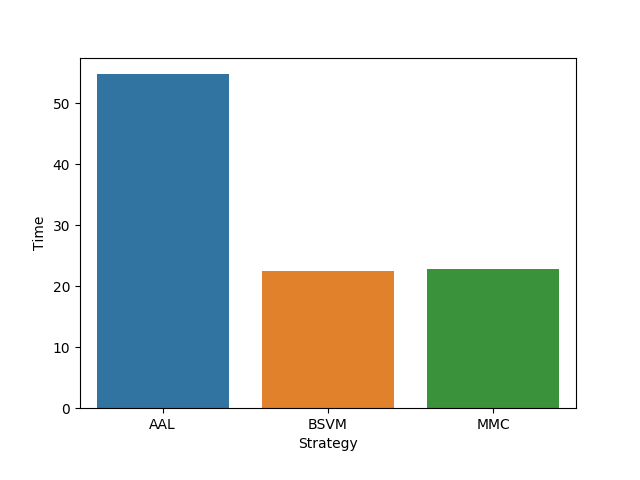
\includegraphics[width=\textwidth]{figures/time-distribution.png}
    \caption{The percentage of time used on the different strategies during one iteration.}
    \label{fig:al-time-dist}
\end{figure}

\section{Experiment 2: Evaluating the Label Balance on the Labeled Dataset}

The goal with the second experiment was to evaluate how the labels in the produced labeled dataset are distributed.
A set where the labels are more evenly, or uniform, distributed would be preferable.
From a perspective of the person labeling, it could feel more productive not assigning the same labels most of the time.
The more prosperous outcome from a balanced dataset would be that the models using the data in later stages could also benefit from this, and obtain better results.
This experiment is used to answer the second research question.

\subsection{Method}

The configurations used here are the same as in Table~\ref{fig:active-learning-configurations}.
Every iteration, the distribution of labels assigned are stored and analyzed.
He et al\@. discusses the usage of ROC curves and measures such as g-means to compare multi-class imbalanced data~\cite{he2009learning}.
However, the doctor involved at Sectra specifically requested that labels should be more uniformly distributed. 
The evaluation will therefore focus on measuring that instead of the models performance, which is done in ~\ref{sec:exp2-method}.
An evaluation of how the distribution progresses was done by comparing how the class imbalance is affected by the number of new samples obtained from the different methods.

Ertekin et al\@.~\cite{ertekin2007learning} used a class imbalance ratio to compare how well an active learning strategy worked.
This was only done for the binary case.
In order to get a measure for the multi-label problem, the evaluation of class imbalance was measured by the percentage of all total labels that were in the most common class, as well as in the top 3 most common classes.
Furthermore, the ratio between the biggest and the smallest class will be used in the evaluation.

This approach is also replicable.
The configurations are clearly defined, and so are the metrics used.
The validity of the experiment is discussed in Section~\ref{sec:sec:discussion-method}.

\subsection{Results}

The results of how the different strategies affected the balance of the labeled dataset is now presented.
For the Reuters dataset, how the overall distribution of the labels is can be seen in Figure~\ref{fig:class-distribution-reuters}.
After random sampling, the distribution can be seen in Figure~\ref{fig:class-distribution-reuters-random}.
For comparison with the techniques it shows the labels both after 500 labels are added, and 2000.
In order to be able to compare it with the other techniques easily, the plot contains the distribution after both 500 and 2000 labels are acquired.
The distribution after sampling with the original BSVM can be seen in Figure~\ref{fig:class-distribution-reuters-binmin}, and with the initial samples taken from clusters in Figure~\ref{fig:class-distribution-reuters-binmin-clusters}.
For MMC the distribution can be seen in Figure~\ref{fig:class-distribution-reuters-mmc}.
The corresponding plots for Adaptive Active Learning can be seen in Figure~\ref{fig:class-distribution-reuters-adaptive} and Figure~\ref{fig:class-distribution-reuters-adaptive-clusters}.

\begin{figure}
    \centering
    \thirdsubfigimg{distribution-RandomSampling-25-500}{The class distribution from random sampling after 500 labels}
    \thirdsubfigimg{distribution-RandomSampling-25-2000}{The class distribution from random sampling after 2000 labels}
    \caption{The distribution of labels after random sampling}
    \label{fig:class-distribution-reuters-random}
\end{figure}

\begin{figure}
    \centering
    \thirdsubfigimg{distribution-BinaryMinimization-25-500}{The class distribution from BSVM after 500 labels}
    \thirdsubfigimg{distribution-BinaryMinimization-25-2000}{The class distribution from BSVM after 2000 labels}
    \caption{The distribution of labels after BSVM}
    \label{fig:class-distribution-reuters-binmin}
\end{figure}


\begin{figure}
    \centering
    \thirdsubfigimg{distribution-ClusterBinaryMinimization-25-500}{The class distribution from BSVM, with the initial sample from clusters, after 500 labels}
    \thirdsubfigimg{distribution-ClusterBinaryMinimization-25-2000}{The class distribution from BSVM, with the initial sample from clusters, after 2000 labels}
    \caption{The distribution of labels after BSVM with clustering}
    \label{fig:class-distribution-reuters-binmin-clusters}
\end{figure}

\begin{figure}
    \centering
    \thirdsubfigimg{distribution-MMC-25-500}{The class distribution from MMC after 500 labels}
    \thirdsubfigimg{distribution-MMC-25-2000}{The class distribution from MMC after 2000 labels}
    \caption{The distribution of labels after MMC}
    \label{fig:class-distribution-reuters-mmc}
\end{figure}

\begin{figure}
    \centering
    \thirdsubfigimg{distribution-AdaptiveLearner-25-500}{The class distribution from Adaptive Active Learning after 500 labels}
    \thirdsubfigimg{distribution-AdaptiveLearner-25-2000}{The class distribution from Adaptive Active Learning after 2000 labels}
    \caption{The distribution of labels after Adaptive Active Learning}
    \label{fig:class-distribution-reuters-adaptive}
\end{figure}

\begin{figure}
    \centering
    \thirdsubfigimg{distribution-ClusterAdaptiveLearner-25-500}{The class distribution from Adaptive Active Learning, with the initial sample from clusters, after 500 labels}
    \thirdsubfigimg{distribution-ClusterAdaptiveLearner-25-2000}{The class distribution from Adaptive Active Learning, with the initial sample from clusters, after 2000 labels}
    \caption{The distribution of labels after Adaptive Active Learning with clustering}
    \label{fig:class-distribution-reuters-adaptive-clusters}
\end{figure}

In Table~\ref{tab:distribution-result-500} the results of the evaluation after 500 new labels can be seen.
The corresponding table for the evaluation after 2000 new labels can be seen in Table~\ref{tab:distribution-result-2000}.

\begin{table}[h!]
    \centering
    \begin{tabular}{|ccccc|}
        \hline
        \textbf{Strategy} & \textbf{Initial Sample} & \textbf{Top Class} & \textbf{Top 3 Classes} & \textbf{Small/Big Ratio}\\
        \hline
        Random & Random &  34.9 \% & 65.5 \% & 32.0 \\
        BSVM & Random &  22.0 \% & 49.8 \% & 45.0 \\
        BSVM & Clusters & 19.8 \% & 49.0 \% & 80.0 \\
        Adaptive & Random & 14.8 \% & 38.5 \% & 5.4 \\
        Adaptive & Clusters & 14.5 \% & 38.2 \% & 6.65 \\
        MMC & Random & 13.1 \% & 35.2 \% & 8.2 \\
        \hline
    \end{tabular}
    \caption{The results after analyzing the label distribution after 500 new labels has been added.}
    \label{tab:distribution-result-500}
\end{table}

\begin{table}[h!]
    \centering
    \begin{tabular}{|ccccc|}
        \hline
        \textbf{Strategy} & \textbf{Initial Sample} & \textbf{Top Class} & \textbf{Top 3 Classes} & \textbf{Small/Big Ratio}\\
        \hline
        Random & Random & 36.65 \% & 64.6 \% & 29.4 \\
        BSVM & Random & 16.0 \% & 42.4 \% & 7.5 \\
        BSVM & Clusters & 15.7 \% & 41.5 \% & 7.3 \\
        Adaptive & Random & 36.4 \% & 56.2 \% & 43.4 \\
        Adaptive & Clusters & 34.5 \% & 54.8 \% & 41.0 \\
        MMC & Random & 16.7 \% & 41.2 \% & 9.3 \\
        \hline
    \end{tabular}
    \caption{The results after analyzing the label distribution after 2000 labels has been added.}
    \label{tab:distribution-result-2000}
\end{table}

\section{Experiment 3: Filtering out Invalid Reports}

This experiment is concerned with the identification of invalid reports.
The task here was to evaluate how well unsupervised techniques could be used to filter out these invalid reports.
Invalid reports are considered to be reports that describe a situation where an examination never took place.
This can be because of a deceased patient, a patient being moved to another hospital, a patient did not show up or for some reason did not want to go through with the examination.
The results of this is the base for answering the third research question.

\subsection{Method}

In order to evaluate how well the selected model performed on the clinical data, a set of reports had to be marked as valid/invalid.
This was done by creating a script that presented a report to the user, and requested the label.
5358 reports were labeled by the author, out of which 623 were marked as invalid. 
In order to make the models able to separate the invalid reports from the valid reports they had to be manually analyzed.
They are both unsupervised methods and were therefore not fitted with a specific target.
Approaching this in a way that would not result in the approach being overfitted to the analyzed data could potentially be hard since they are manually analyzed. 
To reduce the bias in the evaluation, the labeled reports were split into a training set and validation set, containing 80\% and 20\% of the reports respectively.

The training set was further used to be verify the topics that were identified as important, whereas the validation set was used to evaluate how well the approach performed.
This manual identification can be seen in Section~\ref{sec:topic-invalid}.
Based on these findings, reports were determined to be invalid or not based on if they fulfilled both of the following criteria:
\begin{itemize}
    \item Having either topic 1 or 17 as its most probable topic.
    \item Not having more than 6 prominent topics assigned to it.
\end{itemize}
Where prominent topics are defined as those who has a probability of more than 10\% for a given report.


After the initial exploration it was clear that the topic vectors contained patterns ripe for exploitation.
A topic vector is the vector with the topic probabilities for a document.
The patterns are clear enough to motivate the manual identification of topics that are important to differentiate between invalid and valid reports.
In order to compare this result with some more objective baseline, a logistic regression classifier was fitted on the data and evaluated as well.
A set of reports were already labeled with ``invalid'' or ``valid'' in order to evaluate the manual interpretation approach.
This set was thus used to fit the classifier.
The topic vectors were used as features, and the targets were the labels indicating if a report is valid or not.

\subsection{Results}

The evaluation on the validation set can be seen in Table~\ref{tab:exp1-eval}.
In the figure you can also see the results of the logistic regression classifier, which was fitted with the topic vectors as features and the invalid/valid labels as targets.

\begin{table}[h!]
    \centering
    \begin{tabular}{|c|cc|}
        \hline
        & \textbf{Manual topic identification} & \textbf{Logistic regression} \\
        \hline
        \textbf{Precision} & 97.2\% & 98.7\% \\
        \textbf{Recall} & 100\% & 100\% \\
        \textbf{$F_1$-measure} & 98.6\% & 99.4\%\\
        \textbf{Accuracy} & 97.9\% & 99.1\%\\
        \hline
    \end{tabular}
    \caption{The results of the classification of the invalid reports. The manual identification column represents the use of manual interpretation of the LDA topics to find the invalid reports.}
    \label{tab:exp1-eval}
\end{table}

Both of these approaches were evaluated using four different metrics, recall, precision, $F_1$-measure and accuracy.
All of which are described in Section~\ref{sec:evaluation-metrics}.

The replicability of this experiment is varied.
It contains a manual analysis of LDA generated topics, on a proprietary dataset, which may be hard to replicate.
However, performing logistic regression on topic vectors generated with the specific LDA is easier to reproduce.

\section{Frameworks, Tools and Implementation}

The entire system was written in Python.
The motivation behind this choice was mainly that, when it comes to machine learning and text mining, most of the existing infrastructure at Sectra is using Python.
This, in combination with the fact that there exists several tools for these purposes in Python, such as \textit{numpy} \footnote{Numpy, http://www.numpy.org/}, \textit{nltk} \footnote{Natural Language Toolkit, https://www.nltk.org/}, \textit{scikit-learn} \footnote{scikit-learn, http://scikit-learn.org/stable/} and \textit{gensim} \footnote{Gensim, https://radimrehurek.com/gensim/}.
Most of the plotting was done using the \textit{seaborn} \footnote{Seaborn, https://seaborn.pydata.org/} and \textit{bokeh} \footnote{Bokeh, https://bokeh.pydata.org/en/latest/} libraries.
\textit{pyLDAvis} \footnote{pyLDAvis, https://github.com/bmabey/pyLDAvis} was used for some additional visualization purposes with regards to topic models.

However, when it comes to active learning, there does not seem to be a proven mainstream library that contains a set of readily available algorithms.
In order to achieve better integration between the active learning system and the existing infrastructure at Sectra, as well as making adaptions such as the number of items queried in each iteration, an active learning framework was written from scratch.
The ground for this framework were the algorithms presented in Section~\ref{sec:active-learning}.

This framework consisted of three modules, called \textit{model}, \textit{dataset}, and \textit{query strategy}.
The model is a wrapper around different machine learning models.
By providing an interface for a distance or certainty measure, any underlying model able to provide such an interface can be incorporated.
For accessing the data pool a dataset wrapper was written, with an interface for accessing the labeled and unlabeled pools.
Putting this in its own module opens up the possibility for using several different storage solutions, such as a database or plain text files.
The query strategy module contains the different active learning algorithms for selecting what sample to label next.